%+++++++++++++++++++++++++++++++++++++++++++++++++++++++++++++++++++++++++++++++
%+++++++++++++++++++++++++++++++++++++++++++++++++++++++++++++++++++++++++++++++

%\mysubsection{Theory}

This section includes some material on notation, formulations and general theoretical backgrounds for \codeName .
Note that the formulation of nodes, objects, markers, etc. is presented right at the subsection of each object, see \refSection{sec:item:reference:manual}.
Furthermore, overview on the system assembly and system equations of motion is given in \refSection{sec:notationSystemOfEOM},
solvers are described in \refSection{sec:solvers}.

%+++++++++++++++++++++++++++++++++++++++++++++++++++++++++++++++++++++++++++++++++++++++++++
%+++++++++++++++++++++++++++++++++++++++++++++++++++++++++++++++++++++++++++++++++++++++++++
\mysubsection{Notation}
\label{sec:itemnotation}
%
\mysubsubsection{Common types in item descriptions}
%
There are certain types, which are heavily used in the description of items:
\bi
  \item \texttt{float} $\ldots$ a single-precision floating point number (note: in Python, '\texttt{float}' is used also for double precision numbers; in EXUDYN, internally floats are single precision numbers especially for graphics objects and OpenGL)
  \item \texttt{Real} $\ldots$ a double-precision floating point number (note: in Python this is also of type '\texttt{float}')
  \item \texttt{UReal} $\ldots$ same as \texttt{Real}, but may not be negative
  \item \texttt{PReal} $\ldots$ same as \texttt{Real}, but must be positive, non-zero (e.g., step size may never be zero)
  \item \texttt{Index} $\ldots$ deprecated, represents unsined integer, \texttt{UInt}
  \item \texttt{Int} $\ldots$ a (signed) integer number, which converts to '\texttt{int}' in Python, '\texttt{int}' in C++
  \item \texttt{UInt} $\ldots$ an unsigned integer number, which converts to '\texttt{int}' in Python
  \item \texttt{PInt} $\ldots$ an positive integer number (> 0), which converts to '\texttt{int}' in Python
  \item \texttt{NodeIndex, MarkerIndex, ...} $\ldots$ a special (non-negative) integer type to represent indices of nodes, markers, ...; specifically, an unintentional conversion from one index type to the other is not possible (e.g., to convert \texttt{NodeIndex} to \texttt{MarkerIndex})
  \item \texttt{String} $\ldots$ a string
  \item \texttt{ArrayIndex} $\ldots$ a list of integer numbers (either list or in some cases \texttt{numpy} arrays may be allowed)
  \item \texttt{ArrayNodeIndex} $\ldots$ a list of node indices
  \item \texttt{Bool} $\ldots$ a boolean parameter: either \texttt{True} or \texttt{False} ('\texttt{bool}' in Python)
  \item \texttt{VObjectMassPoint}, \texttt{VObjectRigidBody}, \texttt{VObjectGround}, etc.  $\ldots$ represents the visualization object of the underlying object; 'V' is put in front of object name
  \item \texttt{BodyGraphicsData} $\ldots$ see \refSection{sec:graphicsData}
%	
	\item \texttt{Vector2D} $\ldots$ a list or \texttt{numpy} array of 2 real numbers
	\item \texttt{Vector3D} $\ldots$ a list or \texttt{numpy} array of 3 real numbers
	\item \texttt{Vector'X'D} $\ldots$ a list or \texttt{numpy} array of 'X' real numbers
	\item \texttt{Float4} $\ldots$ a list of 4 float numbers
%
	\item \texttt{Vector} $\ldots$ a list or \texttt{numpy} array of real numbers (length given by according object)
	\item \texttt{NumpyVector} $\ldots$ a 1D \texttt{numpy} array with real numbers (size given by according object); similar as Vector, but not accepting list

	\item \texttt{Matrix3D} $\ldots$ a list of lists or \texttt{numpy} array with $3 \times 3$ real numbers
	\item \texttt{NumpyMatrix} $\ldots$ a 2D \texttt{numpy} array (matrix) with real numbers (size given by according object)
	\item \texttt{NumpyMatrixI} $\ldots$ a 2D \texttt{numpy} array (matrix) with integer numbers (size given by according object)
\ei
%
\mysubsubsection{States and coordinate attributes}
The following subscripts are used to define configurations of a quantity, e.g., for a vector of displacement coordinates $\qv$:
\bi
  \item $\qv\cConfig \ldots$ $\qv$ in any configuration
  \item $\qv\cRef \ldots$ $\qv$ in reference configuration, e.g., reference coordinates: $\cv\cRef$
  \item $\qv\cIni \ldots$ $\qv$ in initial configuration, e.g., initial displacements: $\uv\cIni$
  \item $\qv\cCur \ldots$ $\qv$ in current configuration
  \item $\qv\cVis \ldots$ $\qv$ in visualization configuration
  \item $\qv\cSOS \ldots$ $\qv$ in start of step configuration
\ei
As written in the introduction, the coordinates are attributed to certain types of equations and therefore, the following attributes are used (usually as subscript, e.g., $\qv_{ODE2}$):
\bi
  \item \hacs{ODE2} $\ldots$ \acl{ODE2} (coordinates)
  \item \hacs{ODE1} $\ldots$ \acl{ODE1} (coordinates)
  \item \hacs{AE} $\ldots$ \acl{AE} (coordinates)
  \item Data $\ldots$ data coordinates (history variables)
\ei
Time is usually defined as 'time' or $t$.
The cross product or vector product '$\times$' is often replaced by the skew symmetric matrix using the tilde '$\tilde{\;\;}$' symbol,
\be
  \av \times \bv = \tilde \av \, \bv = -\tilde \bv \, \av \eqDot
\ee
For the length of a vector we often use the abbreviation 
\be \label{eq:definition:length}
  \Vert \av \Vert = \sqrt{\av^T \av} \eqDot
\ee
%
%+++++++++++++++++++++++++++++++++++++++++++++++++++++++++++++++++++++++++++++++++++++++++++
\mysubsubsection{Symbols in item equations}
\label{sec:symbolsItems}
\noindent The following table contains the common notation: \vspace{-12pt}
\begin{center}
  \footnotesize
  \begin{longtable}{| p{5cm} | p{5cm} | p{6cm} |}
    \hline
    \bf python name (or description) & \bf symbol & \bf description \\ \hline
    displacement coordinates (\hac{ODE2}) & $\qv = [q_0,\, \ldots,\, q_n]\tp$ & vector of $n$ displacement based coordinates in any configuration; used for second order differential equations\\ \hline
    rotation coordinates (\hac{ODE2}) & $\tpsi = [\psi_0,\, \ldots,\, \psi_\eta]\tp$ & vector of $\eta$ {\bf rotation based coordinates} in any configuration; these coordinates are added to reference rotation parameters to provide the current rotation parameters; used for second order differential equations\\ \hline
    coordinates (\hac{ODE1}) & $\yv = [y_0,\, \ldots,\, y_n]\tp$ & vector of $n$ coordinates for first order ordinary differential equations (\hac{ODE1}) in any configuration\\ \hline
    algebraic coordinates & $\zv = [z_0,\, \ldots,\, z_m]\tp$ & vector of $m$ algebraic coordinates if not Lagrange multipliers in any configuration\\ \hline
    Lagrange multipliers & $\tlambda = [\lambda_0,\, \ldots,\, \lambda_m]\tp$ & vector of $m$ Lagrange multipliers (=algebraic coordinates) in any configuration\\ \hline
    data coordinates & $\xv = [x_0,\, \ldots,\, x_l]\tp$ & vector of $l$ data coordinates in any configuration\\ \hline
%+++++++++++++++++++++++++++++++++++++++++++++++++++
    \hline %new part of table
		\bf python name: OutputVariable & \bf symbol & \bf description \\ \hline
    Coordinate & $\cv = [c_0,\, \ldots,\, c_n]\tp$ & coordinate vector with $n$ generalized coordinates $c_i$ in any configuration; the letter $c$ is used both for \hac{ODE1} and \hac{ODE2} coordinates\\ \hline
    Coordinate\_t & $\dot \cv = [c_0,\, \ldots,\, c_n]\tp$ & time derivative of coordinate vector\\ \hline
    Displacement & $\LU{0}{\uv} = [u_0,\, u_1,\, u_2]\tp$ & global displacement vector with 3 displacement coordinates $u_i$ in any configuration; in 1D or 2D objects, some of there coordinates may be zero\\ \hline
Rotation & $[\varphi_0,\,\varphi_1,\,\varphi_2]\tp\cConfig$ & vector with 3 components of the Euler angles in xyz-sequence ($\LU{0b}{\Rot}\cConfig=:\Rot_0(\varphi_0) \cdot \Rot_1(\varphi_1) \cdot \Rot_2(\varphi_2)$), recomputed from rotation matrix\\ \hline
    %Rotation & $\ttheta = [\theta_0,\, \ldots,\, \theta_n]\tp$ & vector of {\bf rotation parameters} (e.g., Euler parameters, Tait Bryan angles, ...) with $n$ coordinates $\theta_i$ in any configuration\\ \hline
    Identity matrix & $\Im = \mr{1}{0}{0} {0}{\ddots}{0} {0}{0}{1}$ & the identity matrix, very often $\Im = \ImThree$, the $3 \times 3$ identity matrix \\ \hline
    Identity transformation & $\LU{0b}{\ImThree} = \ImThree$ & converts body-fixed into global coordinates, e.g., $\LU{0}{\xv} = \LU{0b}{\ImThree} \LU{b}{\xv}$, thus resulting in $\LU{0}{\xv} = \LU{b}{\xv}$ in this case\\ \hline
    RotationMatrix & $\LU{0b}{\Rot} = \mr{A_{00}}{A_{01}}{A_{02}} {A_{10}}{A_{11}}{A_{12}} {A_{20}}{A_{21}}{A_{22}}$ & a 3D rotation matrix, which transforms local (e.g., body $b$) to global coordinates (0): $\LU{0}{\xv} = \LU{0b}{\Rot} \LU{b}{\xv}$\\ \hline
    RotationMatrixX & $\LU{01}{\Rot_0(\theta_0)} = 
		\mr{1}{0}{0} {0}{\cos(\theta_0)}{-\sin(\theta_0)} {0}{\sin(\theta_0)}{\cos(\theta_0)}$ & rotation matrix for rotation around $X$ axis (axis 0), transforming a vector from frame 1 to frame 0\\ \hline    
    %
		RotationMatrixY & $\LU{01}{\Rot_1(\theta_1)} = 
		\mr{\cos(\theta_0)}{0}{\sin(\theta_0)} {0}{1}{0} {-\sin(\theta_0)}{0}{\cos(\theta_0)}$ & rotation matrix for rotation around $X$ axis (axis 0), transforming a vector from frame 1 to frame 0\\ \hline    %
    RotationMatrixZ & $\LU{01}{\Rot_2(\theta_2)} = 
		\mr{\cos(\theta_0)}{-\sin(\theta_0)}{0} {\sin(\theta_0)}{\cos(\theta_0)}{0} {0}{0}{1}$ & rotation matrix for rotation around $X$ axis (axis 0), transforming a vector from frame 1 to frame 0\\ \hline    
		Position & $\LU{0}{\pv} = [p_0,\, p_1,\, p_2]\tp$ & global position vector with 3 position coordinates $p_i$ in any configuration\\ \hline
		Velocity & $\LU{0}{\vv} = \LU{0}{\dot \uv} = [v_0,\, v_1,\, v_2]\tp$ & global velocity vector with 3 displacement coordinates $v_i$ in any configuration\\ \hline
    AngularVelocity & $\LU{0}{\tomega} = [\omega_0,\, \ldots,\, \omega_2]\tp$ & global angular velocity vector with $3$ coordinates $\omega_i$ in any configuration\\ \hline
    Acceleration & $\LU{0}{\av} = \LU{0}{\ddot \uv} = [a_0,\, a_1,\, a_2]\tp$ & global acceleration vector with 3 displacement coordinates $a_i$ in any configuration\\ \hline
    AngularAcceleration & $\LU{0}{\talpha} = \LU{0}{\dot \tomega} = [\alpha_0,\, \ldots,\, \alpha_2]\tp$ & global angular acceleration vector with $3$ coordinates $\alpha_i$ in any configuration\\ \hline
%
    VelocityLocal & $\LU{b}{\vv} = [v_0,\, v_1,\, v_2]\tp$ & local (body-fixed) velocity vector with 3 displacement coordinates $v_i$ in any configuration\\ \hline
    AngularVelocityLocal & $\LU{b}{\tomega} = [\omega_0,\, \ldots,\, \omega_2]\tp$ & local (body-fixed) angular velocity vector with $3$ coordinates $\omega_i$ in any configuration\\ \hline
    Force & $\LU{0}{\fv} = [f_0,\, \ldots,\, f_2]\tp$ & vector of $3$ force components in global coordinates\\ \hline
    Torque & $\LU{0}{\ttau} = [\tau_0,\, \ldots,\, \tau_2]\tp$ & vector of $3$ torque components in global coordinates\\ \hline
%+++++++++++++++++++++++++++++++++++++++++++++++++++
		\hline %new part of table
    \bf python name: input to nodes, markers, etc. & \bf symbol & \bf description \\ \hline
    referenceCoordinates & $\cv\cRef = [c_0,\, \ldots,\, c_n]\cRef\tp = [c_{\mathrm{Ref},0},\, \ldots,\, c_{\mathrm{Ref},n}]\cRef\tp$ & $n$ coordinates of reference configuration (can usually be set at initialization of nodes)\\ \hline
    initialCoordinates & $\cv\cIni$ & initial coordinates with generalized or mixed displacement/rotation quantities (can usually be set at initialization of nodes)  \\ \hline
    reference point & $\pRefG = [r_0,\, r_1,\, r_2]\tp$ & reference point of body, e.g., for rigid bodies or \hac{FFRF} bodies, in any configuration; NOTE: for ANCF elements, $\pRefG$ is used for the position vector to the beam centerline\\ \hline    
    localPosition & $\pLocB = [\LUR{b}{b}{0},\, \LUR{b}{b}{1},\, \LUR{b}{b}{2}]\tp$ & local (body-fixed) position vector with 3 position coordinates $b_i$ in any configuration, measured relative to reference point; NOTE: for rigid bodies, $\LU{0}{\pv} = \pRefG + \LU{0b}{\Rot} \pLocB$;
		localPosition is used for definition of body-fixed local position of markers, sensors, COM, etc.\\ \hline
	  \end{longtable}
	\end{center}
%
%+++++++++++++++++++++++++++++++++++++++++++++++++++++++++++++++++++++++++++++++++++++++++++
%+++++++++++++++++++++++++++++++++++++++++++++++++++++++++++++++++++++++++++++++++++++++++++
\mysubsubsection{Reference and current coordinates}
%
An important fact on the coordinates is upon the splitting of quantities (e.g. position, rotation parameters, etc.) into reference and current (initial/visualization/...) coordinates.
The current position vector of a point node is computed from the reference position plus the current displacment, reading
\be
  \pv\cCur = \pv\cRef + \uv\cCur
\ee
In the same way rotation parameters are computed from,
\be
  \ttheta\cCur = \ttheta\cRef + \tpsi\cCur
\ee
which are based on reference quantities plus displacements or {\it changes}. Note that these changes are additive, even for rotation parameters. Needless to say, $\tpsi\cCur$ do not represent rotation parameters, while $\ttheta\cRef$ should be chosen such that they represent the orientation of a node in reference configuration.
The necessity for reference coordinates originates from finite elements, which usually split nodal position into displacements and reference position.
However, we also use the reference position here in order to define joints, e.g., using the utility function \texttt{AddRevoluteJoint(...)}.

Against to the splitting of positions, displacements and velocities (and most other quantities) are not having this reference part!

\mysubsubsection{Reference point}
%
In contrast to the reference position or reference coordinates, the reference point is mainly used for objects, e.g., rigid bodies.
The reference point is the position of the underlying (rigid body) node, while we can compute the position of any point on the body (or on the mass point).
The reference point is also the origin of the co-rotating (reference) frame with the body-fixed coordinate system.

The same concept is also used for \hac{FFRF} objects. In most cases, reference points are denoted by $\pRef$.

%+++++++++++++++++++++++++++++++++++++++++++++++++++++++++++++++++++++++++++++++++++++++++++
\mysubsubsection{Coordinate Systems}
%
\noindent The left indices provide information about the coordinate system, e.g.,
\be
  \LU{0}{\uv}
\ee
is the displacement vector in the global (inertial) coordinate systme $0$, while 
\be
  \LU{m1}{\uv}
\ee
represents the displacement vector in marker 1 ($m1$) coordinates. Typical coordinate systems:
\bi
  \item $\LU{0}{\uv}$ $\ldots$ global coordinates
  \item $\LU{b}{\uv}$ $\ldots$ body-fixed, local coordinates
  \item $\LU{m0}{\uv}$ $\ldots$ local coordinates of (the body or node of) marker $m0$
  \item $\LU{m1}{\uv}$ $\ldots$ local coordinates of (the body or node of) marker $m1$
  \item $\LU{J0}{\uv}$ $\ldots$ local coordinates of joint $0$, related to marker $m0$
  \item $\LU{J1}{\uv}$ $\ldots$ local coordinates of joint $1$, related to marker $m1$
\ei
To transform the local coordinates $\LU{m0}{\uv}$ of marker 0 into global coordinates $\LU{0}{\xv}$, we use
\be
  \LU{0}{\uv} = \LU{0,m0}{\Rot} \LU{m0}{\uv}
\ee
in which $\LU{0,m0}{\Rot}$ is the transformation matrix of (the body or node of) the underlying marker 0.





%+++++++++++++++++++++++++++++++++++++++++++++++++++++++++++++++++++++++++++++++++++++++++++
\newpage
\mysubsection{Model order reduction and \hac{CMS}}
\label{sec:theory:CMS}
%terminology: eigenmode, eigenvector, eigenvalue, normal mode, static mode

This section describes the process how to create general flexible multibody system models using the floating frame of reference formulation with model order reduction (here also denoted as \hac{CMS}). The according object \texttt{ObjectFFRFreducedOrder} is described in \refSection{sec:item:ObjectFFRFreducedOrder}.

\mysubsubsection{Eigenmodes}
This section will describe the computation of eigenmodes using FEMinterface.

The \texttt{FEMinterface} in the module \texttt{FEM} has various functionality to import finite element meshes from finite element software.
We create a \texttt{FEMinterface} by means of
\bi
  \item[] \texttt{fem = FEMinterface()}
\ei
which allows us to use the variable \texttt{fem} from now.

Meshes can be imported from NETGEN/NGsolve (\refSection{sec:FEM:FEMinterface:ImportMeshFromNGsolve}), Abaqus (see \refSection{sec:FEM:FEMinterface:ImportFromAbaqusInputFile} and other sections related to ABAQUS), ANSYS (see \refSection{sec:FEM:FEMinterface:ReadElementsFromAnsys} and other sections related to ANSYS).
The import procedure, which can also be done manually, needs to include \texttt{massMatrix} $\Mm$ and \texttt{stiffnessMatrix} $\Km$ from any finite element model.
Note that many functions are based on the requirement that nodes are 3D displacement-based nodes, without rotation or other coordinates.

For any functionality with \texttt{ObjectFFRFreducedOrder} and for the computation of Hurty-Craig-Bampton modes as described in the next section, \texttt{nodes}
are required.
Finally, \texttt{elements} need to be included for visualization, and a surface needs to be reconstructed from the element connectivity, which is available for tetrahedral and hexahedral elements for most import functions.

%++++++++++++++++++++++++
\begin{figure}[tbph]
  \begin{center}
  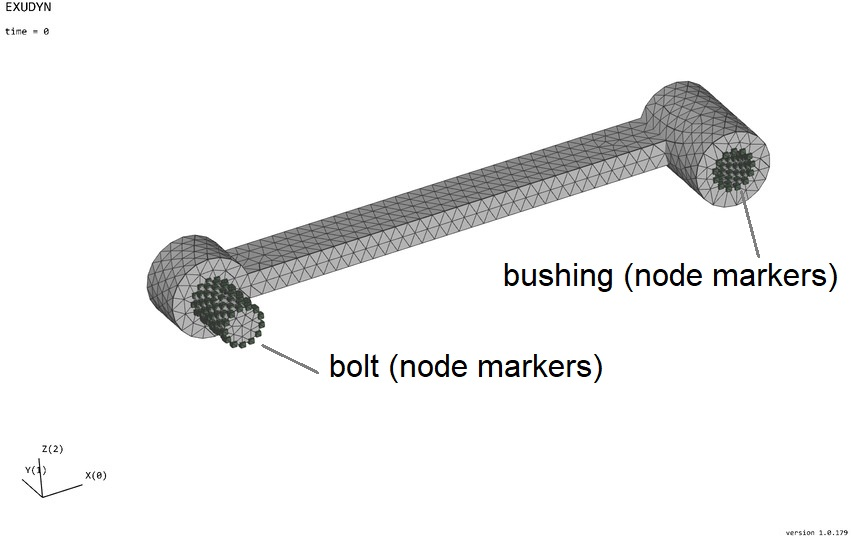
\includegraphics[width=10cm]{figures/modesHinge/HCBhingeMesh.jpg}
  \end{center}
  \caption{Test model and mesh for hinge created with Netgen (linear tetrahedral elements).}
	\label{fig_hingePartMesh}
\end{figure}
%++++++++++++++++++++++++
As an example, we consider a part denoted as 'hinge' in the following, see \fig{fig_hingePartMesh}. The test example can be found in \texttt{Examples/NGsolveCMStutorial.py} with lots of additional features.

After import of mass and stiffness matrix, eigenmodes and eigenfrequencies can be computed using \texttt{fem.ComputeEigenFrequencies(...)}, 
which computes the quantities \texttt{fem.modeBasis} and \texttt{fem.eigenValues}.
The eigenvalues in Hz can be retrieved also with the function \texttt{fem.GetEigenFrequenciesHz()}.
The function \texttt{fem.ComputeEigenFrequencies(...)} is available for dense and sparse matrices, and uses \texttt{scipy.linalg} to compute eigenvalues of the linear, undamped mechanical system
\be \label{theory:eigenmodes:EOM}
	\Mm \ddot \qv(t) + \Km \qv(t) = \fv(t) \eqDot
\ee
Here, the total number of coordinates of the system is $n$, 
thus having the vector of system coordinates $\qv \in \Rcal^n$, 
vector of applied forces $\fv \in \Rcal^n$, 
mass matrix $\Mm \in \Rcal^{n \times n}$ and stiffness matrix $\Km \in \Rcal^{n \times n}$. 
If we are interested in free vibrations of the system, without any boundary conditions or interconnections to other bodies, \eq{theory:eigenmodes:EOM} can be converted to a generalized eigenvalue problem. Using the approach 
$\qv(t) = \vv \mathrm{e}^{\mathrm{i} \omega t}$ in \eq{theory:eigenmodes:EOM}, and thus $\ddot \qv(t) = -\omega^2 \qv(t)$, we obtain
\be \label{theory:eigenmodes:harmonicEquation}
		\left[ \left(-\omega^2 \Mm + \Km \right) \vv \right] \mathrm{e}^{i\omega t} = \Null \eqDot
\ee
Assuming that \eq{theory:eigenmodes:harmonicEquation} is valid for all times, the {\bf generalized eigenvalue problem} follows that
\be \label{theory:eigenmodes:GEP}
	\left(-\omega^2 \Mm + \Km \right) \vv = \Null \eqComma
\ee
which can be rewritten as
\be \label{theory:eigenmodes:GEP2}
	\det \left(-\omega^2 \Mm + \Km \right) = 0 \eqComma
\ee
and which defines the eigenvalues $\omega_i^2$ of the linear system, where $i \in \{0, \ldots, n-1\}$. Note that in this case, the eigenvalues are the squared eigenfrequencies (in rad/s).
We can use eigenvalue algorithms to compute the eigenvalues $\omega_i^2$ and according eigenvectors $\vv_i$ from Python.
The function \texttt{fem.ComputeEigenmodes(...)} uses \texttt{eigh(...)} from \texttt{scipy.linalg} in the dense matrix mode, 
and in the sparse mode \texttt{eigsh(...)} from \texttt{scipy.sparse.linalg}, the latter being restricted to pure symmetric matrices.
Using special shift-inverted techniques in \texttt{eigsh(...)}, it performs much better than standard settings. However, you may tune your specific eigenvalue problem by modifying the solver procedure (just copy that function and adjust to your needs).
As an output, we obtain the smallest \texttt{nModes} eigenvectors (=eigenmodes)\footnote{Eigenvectors are the result of the eigenvalue algorithm, such as the QR algorithm. The mechanical interpretation of eigenvectors are eigenmodes, that can be visualized as shown in the figures of this section.} of the system.
Here, we will also use synonymously the terms `eigenmodes' and `normal modes', which result from an eigenvalue/eigenvector computation using certain (or even no) boundary conditions.
%++++++++++++++++++++++++
\begin{figure}[tbph]
  \begin{center}
  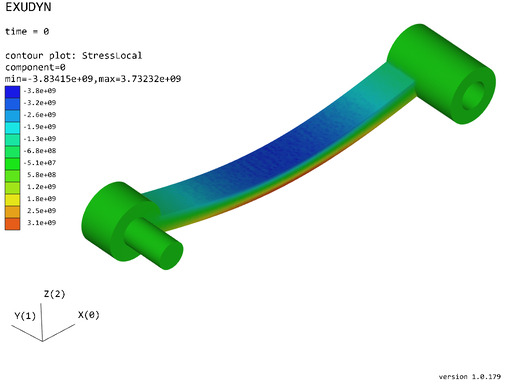
\includegraphics[width=4cm]{figures/modesHinge/freeFreeModeStress1}
  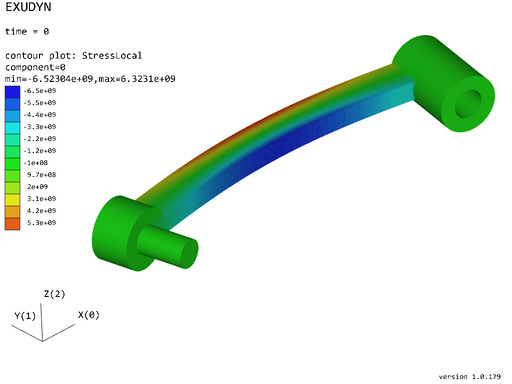
\includegraphics[width=4cm]{figures/modesHinge/freeFreeModeStress2}
  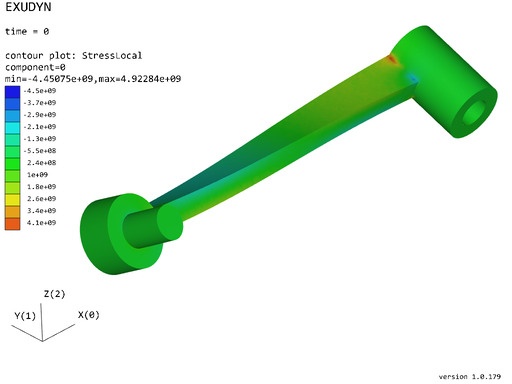
\includegraphics[width=4cm]{figures/modesHinge/freeFreeModeStress3}
  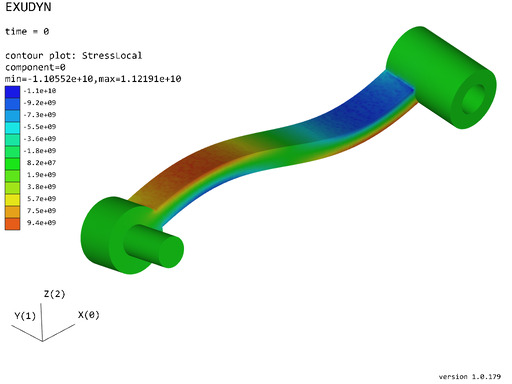
\includegraphics[width=4cm]{figures/modesHinge/freeFreeModeStress4}\\
  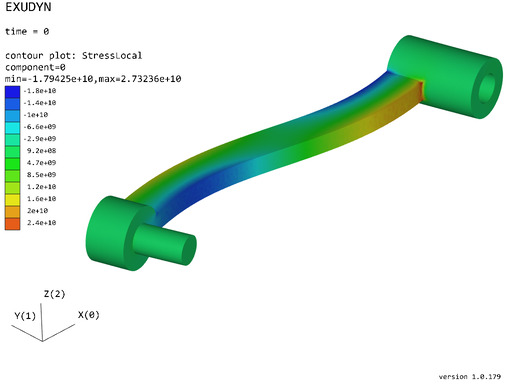
\includegraphics[width=4cm]{figures/modesHinge/freeFreeModeStress5}
  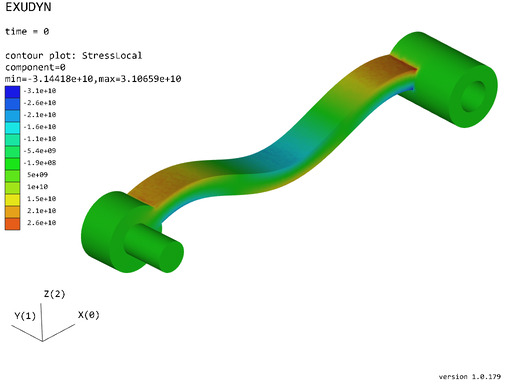
\includegraphics[width=4cm]{figures/modesHinge/freeFreeModeStress6}
  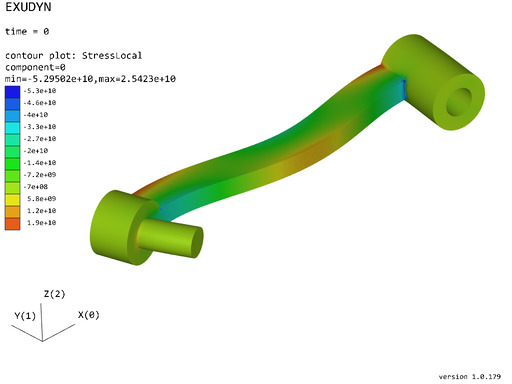
\includegraphics[width=4cm]{figures/modesHinge/freeFreeModeStress7}
  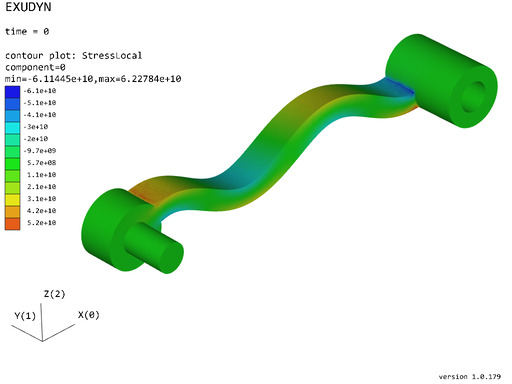
\includegraphics[width=4cm]{figures/modesHinge/freeFreeModeStress8}
  \end{center}
  \caption{Lowest 8 free-free modes for hinge finite element model, contour plot for $xx$-stress component.}
	\label{fig_hingePartFreeFreeModes}
\end{figure}
%++++++++++++++++++++++++

Clearly, if there are no supports included in the stiffness matrix, the resulting eigenmodes will contain 6 rigid body modes and we will also call this case for the computation of eigenmodes the `free-free' case, in analogy to a simply supported beam.
This rigid body modes, which are usually not needed (=unwanted) in the succeeding computation, can be excluded with an according option in \vspace{6pt}\\
\texttt{fem.ComputeEigenFrequencies(excludeRigidBodyModes = ...)}
\vspace{12pt}\\
For our test example, 8 eigenmodes are shown in \fig{fig_hingePartFreeFreeModes}, where the 6 rigid body modes have been excluded (so in total, 14 eigenvectors were computed).
%free free modes (coarse mesh, nNodes= 1216):
%freq(Hz)=[ 671.59137506  707.17488417 1298.50905491 1929.97563131 1971.76505866
%3141.47119938 3595.34508711 4317.51987533]
The 8 eigenfrequencies for the chosen coarse mesh with mesh size $h=0.01$ and 1216 nodes result as 
\be
  f_{0..7} = [ 671.59, 707.17, 1298.50, 1929.97, 1971.76, 3141.47, 3595.34, 4317.51] Hz
\ee
Note, that a computation with a finer mesh, using mesh size $h=0.002$ and 100224 nodes, leads to significantly different eigenfrequencies, starting with $f_0=371.50\,$Hz. This shows that quadratic finite elements would be more appropriate for this case.

After the computation of modes, it is always a good idea to visualize and/or animate these modes. We can do this, using the function \texttt{AnimateModes(...)} available in \texttt{exudyn.interactive}, which allows us to inspect and animate modes and to create animations for these modes, see the mentioned example.

Clearly, the free-free modes in \fig{fig_hingePartFreeFreeModes} are not well suited for the modeling of the deformations within the hinge, if the bolt and the bushing shall be fixed to ground or to another part. 
%TO BE DONE:
%We investigate this by adding a simple revolute joint to the bolt.
Therefore, we can use modes based on ideas of Hurty \cite{Hurty1965} and Craig-Bampton \cite{CraigBampton1968}, as shown in the following.


%+++++++++++++++++++++++++++++++++++++++++++++++++++++++++++++++++++++++++++++++++++++++++++++++++++++++++++++++++++++++
%+++++++++++++++++++++++++++++++++++++++++++++++++++++++++++++++++++++++++++++++++++++++++++++++++++++++++++++++++++++++
%+++++++++++++++++++++++++++++++++++++++++++++++++++++++++++++++++++++++++++++++++++++++++++++++++++++++++++++++++++++++
\mysubsubsection{Hurty-Craig-Bampton modes}
This section will describe the computation of static and eigen (normal) modes using FEMinterface.
The theory is based on Hurty \cite{Hurty1965} and Craig-Bampton \cite{CraigBampton1968}, but often only attributed to Craig-Bampton.
Furthermore, boundaries are also called interfaces\footnote{Here, and in the description of various Python functions, we will use boundary and interface often synonymously, as flexible bodies can be either connected to ground in the sense of a classical 'support-type' boundary condition, or they can represent the boundary of the flexible body as an interface to joints (via markers).}, as they either represent surface sections of our finite element model which are connected to the ground or they represent interfaces to joints and are connected to other bodies.

The computation of so-called static and normal modes follows a simple concept based on finite element mass and stiffness matrices.
The final goal of the computation of modes is to approximate the solution $\qv \in \Rcal^n$ 
by means of a reduction basis $\tPsi \in \Rcal^{n \times m}$ 
and a reduced set of coordinates $\pv \in \Rcal^m$, for which we assume $m \ll n$.

In order to include boundary/interface effects, we separate our nodes and the nodal coordinates into 
\bi
  \item[] a) boundary nodes $\qv_b \in \Rcal^{n_b}$ and
	\item[] b) internal or inner nodes $\qv_i \in \Rcal^{n_i}$.
\ei
We assume that internal nodes are not exposed to boundary/interface conditions or to forces.

Therefore, we may rewrite \eq{theory:eigenmodes:EOM} as follows
\be \label{eq_GuyanIrons}
	\mp{\Mm_{bb}}{\Mm_{bi}}{\Mm_{ib}}{\Mm_{ii}} \vp{\ddot{\qv}_b}{\ddot{\qv}_i} + \mp{\Km_{bb}}{\Km_{bi}}{\Km_{ib}}{\Km_{ii}} \vp{\qv_b}{\qv_i} =   \vp{\fv_b}{\Null}
\ee
or, equivalently,
\bea
	\Mm_{bb} \ddot{\qv}_b + \Mm_{bi} \ddot{\qv}_i +\Km_{bb}  {\qv}_b + \Km_{bi}  {\qv}_i  = {\fv}_b \label{eq_Guyan_bb}\\
	\Mm_{ib} \ddot{\qv}_b + \Mm_{ii} \ddot{\qv}_i +\Km_{ib}  {\qv}_b + \Km_{ii}  {\qv}_i  = \Null \eqDot \label{eq_Guyan_ii}
\eea
A pure static condensation follows from \eq{eq_Guyan_ii} with the assumption that inertia terms are neglected,
leading to the static result for internal nodes,
\be 
	{\qv}_{i,stat}=-\Km_{ii}^{-1} \Km_{ib} {\qv}_{b} \eqDot 
\ee
A pure static condensation, also denoted as Guyan-Irons method, keeps boundary coordinates but removes all internal modes, using the approximation
\be
	\label{eq_guans_red}
	\vp{\qv_b}{\qv_i} \approx \vp{\Im}{-\Km_{ii}^{-1} \Km_{ib}}  \qv_b = \tPsi^{GI} \qv_b \eqComma
\ee
which leads to no approximations ('exact') results for the static case, but poor performance in highly dynamic problems.

Significant improvement result from the Hurty-Craig-Bampton method, which adds eigenmodes of the internal coordinates (internal nodes).
We assume that $\tPsi_{ii}$ is the matrix of eigenvectors as a solution to the eigenvalue problem
\be \label{theory:eigenmodes:GEPii}
	\left(-\omega^2 \Mm_{ii} + \Km_{ii} \right) \vv = \Null \eqComma
\ee
Hereafter, we will only keep the lowest (or other appropriate) $m$ eigenmodes in a reduced eigenmode matrix,
\be
  \tPsi^{(red)}_{ii} = \left[\tPsi_{ii,0}, \ldots, \tPsi_{ii,m-1} \right]
\ee
Combining these `fixed-fixed' eigenvectors with the Guyan-Irons reduction \eqref{eq_guans_red}, we obtain the 
Hurty-Craig-Bampton modes as
\be
	\vp{\qv_b}{\qv_i} \approx \vp{\Im}{-\Km_{ii}^{-1} \Km_{ib}}  \qv_b  +  \vp{\Null}{\tPsi_{r,i}}  \pv_{r} \eqComma
\ee
or in matrix form
\be \label{theory:eigenmodes:HCB}
	\vp{\qv_b}{\qv_i} \approx \mp{\Im}{\Null}{-\Km_{ii}^{-1} \Km_{ib}}{\tPsi_{r,i}}   \vp{\qv_b}{\pv_r} = \tPsi^{HCB} \pv^{HCB} \eqDot
\ee
The disadvantage of \eq{theory:eigenmodes:HCB} is evident by the fact that there may be a large number of boundary/interface nodes, leading to a huge number of static modes (100s or 1000s) and thus making the model reduction inefficient. Therefore, we can switch to other interfaces, as described in the following.

\mysubsubsubsection{Definition of RBE2 interfaces}
A powerful extension, which is available in many finite element as well as flexible multibody codes, is the definition of special boundary/interface conditions, based on pure rigid body motion.
The so-called RBE2 boundaries are defined such that they are firmly connected to a rigid frame, thus the boundary or interface can only undergo rigid body motion.
The advantage of this procedure is that, in comparison to \eq{theory:eigenmodes:HCB}, the number of boundary/interface modes is given by 6 {\it rigid body} modes, which allow simple integration into standard joints of multibody systems, e.g., the \texttt{GenericJoint}.
The disadvantage is that such modes usually lead to artificial stiffening and stresses close to the boundary.

\mysubsubsubsection{Computation of Hurty-Craig-Bampton modes with RBE2 interfaces}
In the following section, we show the procedure for the computation of static modes for the RBE2 rigid-body interfaces.

First, we use the index $j$ here as a node index, having the clear correspondence to the coordinate index $i$, that node $j$ has coordinates 
$[3\cdot j,\; 3\cdot j+1,\; 3\cdot j+2]$.
Furthermore, nodes are split into boundary and internal nodes, which then leads to according internal and boundary coordinates.
We shall note that this sorting is never done in the finite element model or matrices, but just some indexing (referencing) lists are generated and used throughout, using valuable features of \texttt{numpy.linalg} and \texttt{scipy.sparse}.

For a certain boundary node set $B=[j_0, \; j_1, \; j_2, \; ...] \in \Ncal^{n_b}$ with certain $n_b$ node indices $j_0, ...$, we define one boundary set. The following transformations need to be performed for every set of boundary node lists. We also assume that weighting of all boundary nodes is equal, which may not be appropriate in all cases.

If we assume that there may only occur rigid body translation and rotation for the whole boundary node set, which is according to the idea of so-called RBE2 boundary conditions, it follows that the translation of all boundary nodes is given by
\be
  \Tm_t = \left[ \Im \; \Im \; \ldots \; \Im \right]\tp \in \Rcal^{3 n_b \times 3}
\ee
with $\Im \in \Rcal^{3\times 3}$ identity matrices. 
The nodal translation coordinates on boundary $B$ are denoted as $\qv_{B,t} \in \Rcal^3$. The translation of the boundary/interface is mapped to the boundary coordinates as follows (assuming only one boundary $B$),
\be
  \qv_{b,t} = \Tm_t \, \qv_{B,t}
\ee
The nodal rotation coordinates on boundary $B$ are denoted as $\qv_{B,r} \in \Rcal^3$. The rotation of the boundary/interface is mapped to the boundary coordinates as follows (assuming only one boundary $B$),
\be
  \qv_{b,r} = \Tm_r \, \qv_{B,r}
\ee
The computation of matrix $\Tm_r$ is more involved. It is based on nodal (reference) position vectors $\rv^{(0)}_j$, $j \in B$, 
the midpoint of all boundary nodes, 
\be
  \rv^{(m)} = \frac{1}{n_b} \sum_{j=0}^{n_b-1} \rv^{(0)}_j
\ee
and the position relative to the midpoint, denoted as 
\be
  \rv_j = \rv^{(0)}_j - \rv^{(m)} \eqDot
\ee
The transformation for rotation follows from 
\be
  \Tm_r  = \left[ \widetilde \tOmega_x \rv_{j_0} \;\; \widetilde \tOmega_y \rv_{j_0} \;\; \widetilde \tOmega_z \rv_{j_0} \;\;
	                \widetilde \tOmega_x \rv_{j_1} \;\; \widetilde \tOmega_y \rv_{j_1} \;\; \widetilde \tOmega_z \rv_{j_1}
									\ldots \right]\tp \in \Rcal^{3 n_b \times 3}
\ee
with the special tensors, representing rotation about (x,y,z)-axes,
\be
  \widetilde\tOmega_x = \mr{0}{0}{0} {0}{0}{-1} {0}{1}{0}, \quad
  \widetilde\tOmega_y = \mr{0}{0}{1} {0}{0}{0} {-1}{0}{0}, \quad
  \widetilde\tOmega_z = \mr{0}{-1}{0} {1}{0}{0} {0}{0}{0} \eqDot
\ee

The total nodal coordinates at the boundary, representing translations and rotations, follow as
\be
  \qv_{B} = \vp{\qv_{B,t}}{\qv_{B,r}} \eqComma
\ee
and the transformation matrix for the translation and rotation simply reads
\be
  \Tm = [\Tm_t \;\; \Tm_r] \in \Rcal^{3n_b \times 6} \eqComma
\ee
which provides the total mapping of boundary rigid body motion
\be
  \qv_{b} = \Tm \, \qv_{B} \eqComma
\ee 
which is the sum of translation and rotation.

As an example, having the boundary nodes sorted for two boundary node set $B_0$ and $B_1$, we obtain the following transformation for the Hurty-Craig-Bampton method with only 6 modes per boundary node set,
\be \label{theory:eigenmodes:HCBRBE2}
	%\vp{\qv_b}{\qv_i} \approx \mp{ \Im \mp{\Tm_0}{}{}{\Tm_1}}{\Null}{-\Km_{ii}^{-1} \Km_{ib}\vp{\Tm_0}{\Tm_1}}{\tPsi_{r,i}}   
	%\vr{\qv_{B_0}}{\qv_{B_1}}{\pv_r} \eqDot
	\vp{\qv_b}{\qv_i} \approx \mr{ \Tm_0}{\Null}{\Null} {\Null}{\Tm_1}{\Null} 
	                          {-\Km_{ii}^{-1} \Km_{ib}\vp{\Tm_0}{\Null} }{-\Km_{ii}^{-1} \Km_{ib}\vp{\Null}{\Tm_1} }{\tPsi_{r,i}}   
	\vr{\qv_{B_0}}{\qv_{B_1}}{\pv_r} \eqDot
\ee
with the new boundary node vector $\qv_b = [\qv_{B_0}\tp \;\; \qv_{B_1}\tp]\tp$.
%\newcommand{\mr}[9]{\left[\!\! \begin{array}{ccc} #1 & #2 & #3 \vspace{0.1cm}\\ #4 & #5 & #6 \vspace{0.1cm}\\ #7 & #8 & #9  \end{array} \!\!\right]}

{\bf Notes}:
\bi
  \item The inverse $\Km_{ii}^{-1} $ is not computed, but this matrix is LU-factorized using sparse techniques.
	\item The factorization only needs to be applied to six vectors for every relevant boundary node set.
	\item One set of boundary nodes can be omitted from the final static modes in \eq{theory:eigenmodes:HCBRBE2}, because keeping all boundary modes, would introduce six rigid body motions to our mode basis, what is usually not wanted nor needed.
\ei

Using again the examples given in \fig{fig_hingePartMesh}, we now obtain a set of modified modes using the function \texttt{fem.ComputeHurtyCraigBamptonModes(...)}.
\fig{fig_hingePartStaticModesA} shows the first 6 rigid body modes. Note that these modes would be automatically removed in the function \texttt{fem.ComputeHurtyCraigBamptonModes(...)}.
\fig{fig_hingePartStaticModesB} shows the second set of 6 rigid body modes. 
Finally, 8 eigenmodes have been computed for the fixed-fixed case (where all boundary/interfaces nodes are fixed),
see \fig{fig_hingePartFixedFixedModes}. 
The eigenfrequencies for this case now are significantly higher than in the free-free case, reading
\be
  f_{0..7} = [1277.35, 1469.86, 3336.91, 3584.28, ...]
\ee
%Hurty-Craig-Bampton modes (coarse mesh, nNodes= 1216):
 %freq(Hz)=[1277.35052832 1469.86514681 3336.91168906 3584.28464361 5079.65220372
 %6035.58805197 6049.99829894 6568.47108075]
%++++++++++++++++++++++++
\begin{figure}[tbph]
  \begin{center}
  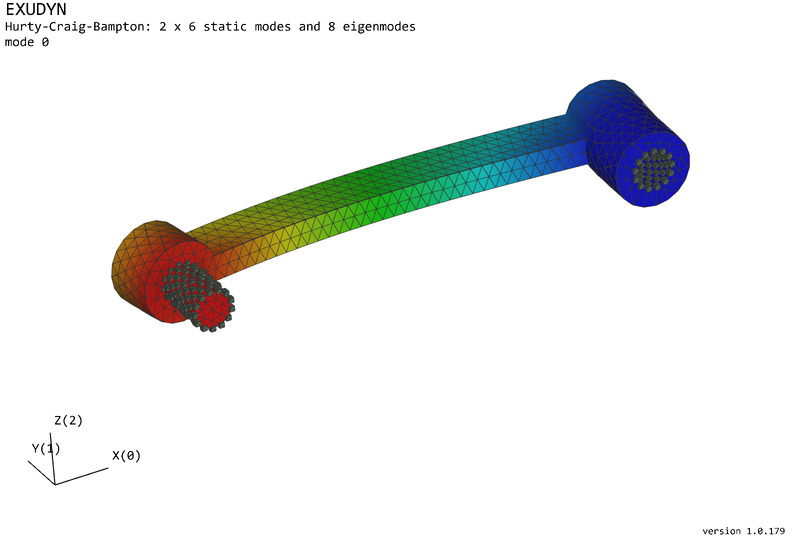
\includegraphics[width=5cm]{figures/modesHinge/HCBmodesHingeStaticAx}
  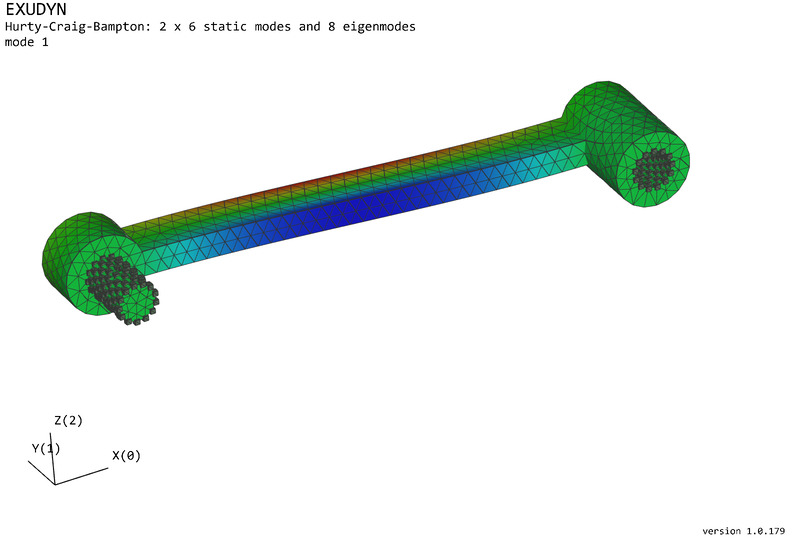
\includegraphics[width=5cm]{figures/modesHinge/HCBmodesHingeStaticAy}
  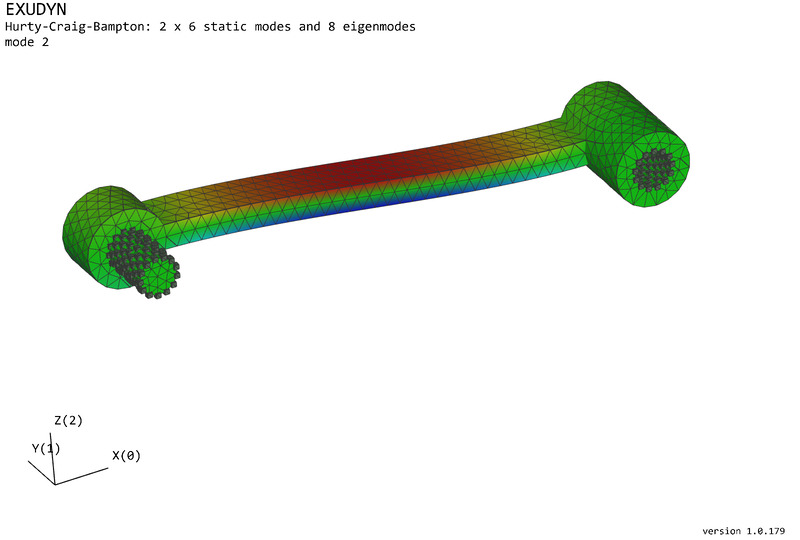
\includegraphics[width=5cm]{figures/modesHinge/HCBmodesHingeStaticAz}\\
  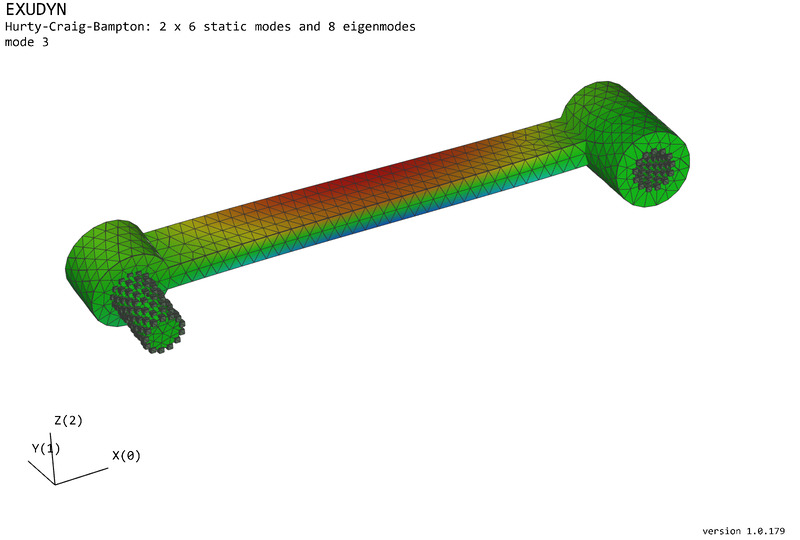
\includegraphics[width=5cm]{figures/modesHinge/HCBmodesHingeStaticArotX}
  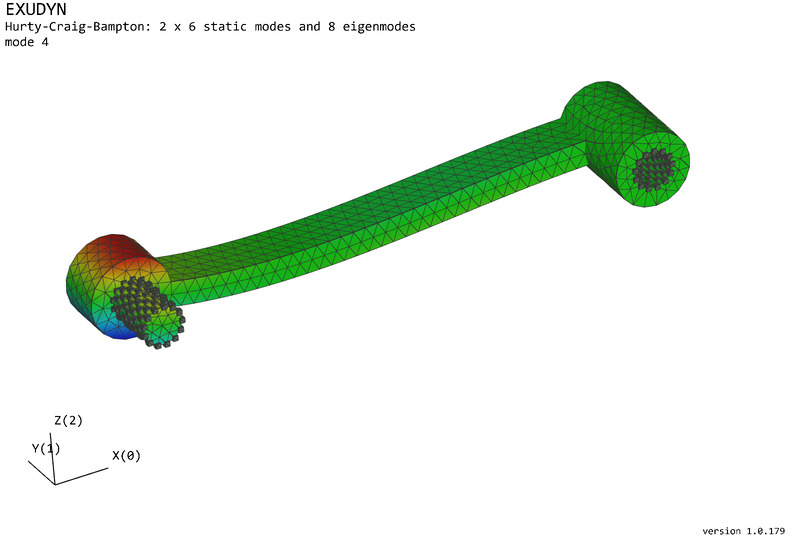
\includegraphics[width=5cm]{figures/modesHinge/HCBmodesHingeStaticArotY}
  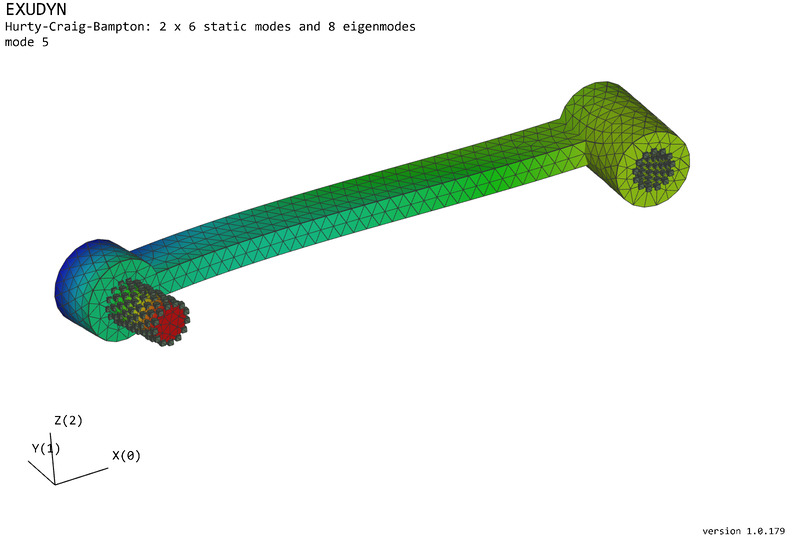
\includegraphics[width=5cm]{figures/modesHinge/HCBmodesHingeStaticArotZ}
  \end{center}
  \caption{Static modes for bolt rigid body interface, using Hurty-Craig-Bampton method; top three images show (x,y,z)-translation modes, bottom three images show (x,y,z)-rotation modes; contour color represents norm of displacements.}
	\label{fig_hingePartStaticModesA}
\end{figure}
%++++++++++++++++++++++++

%++++++++++++++++++++++++
\begin{figure}[tbph]
  \begin{center}
  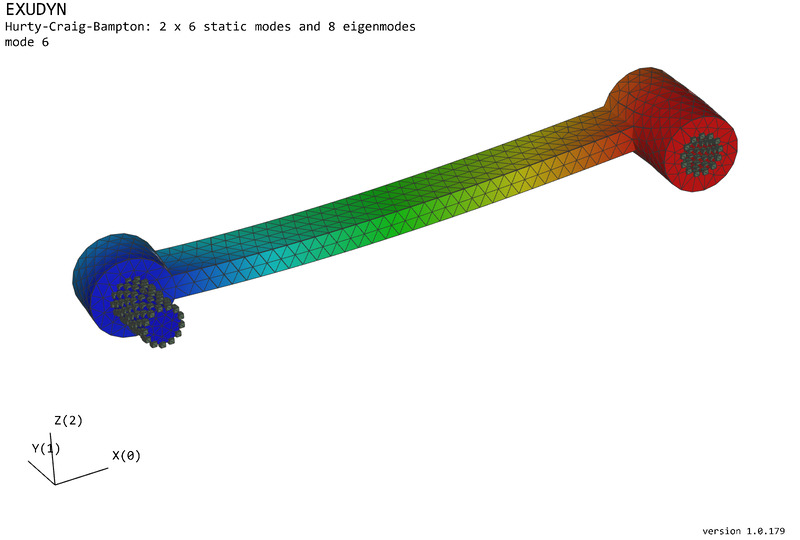
\includegraphics[width=5cm]{figures/modesHinge/HCBmodesHingeStaticBx}
  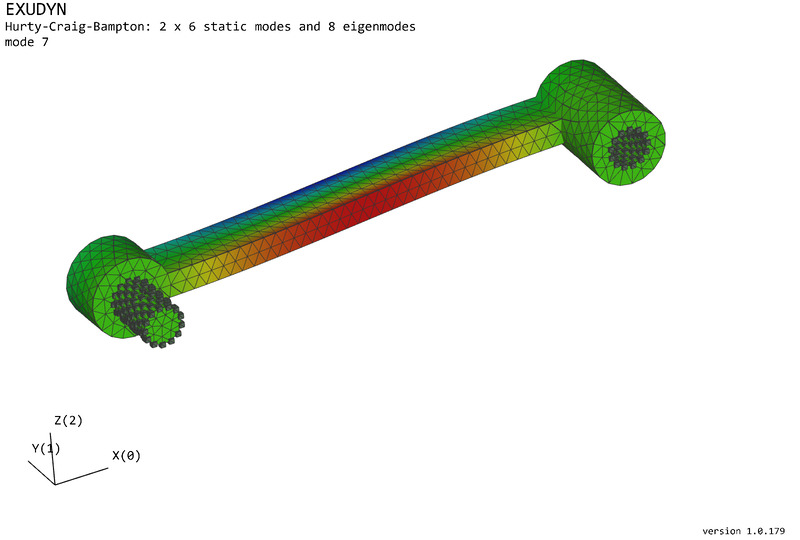
\includegraphics[width=5cm]{figures/modesHinge/HCBmodesHingeStaticBy}
  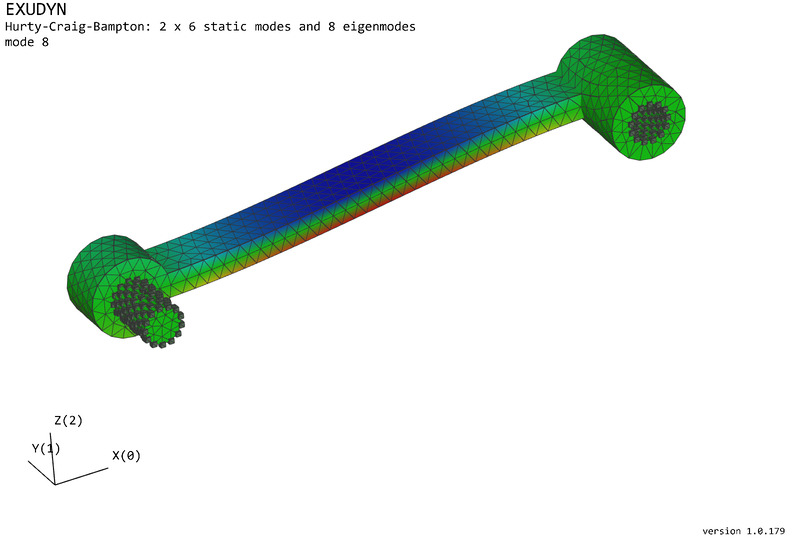
\includegraphics[width=5cm]{figures/modesHinge/HCBmodesHingeStaticBz}\\
  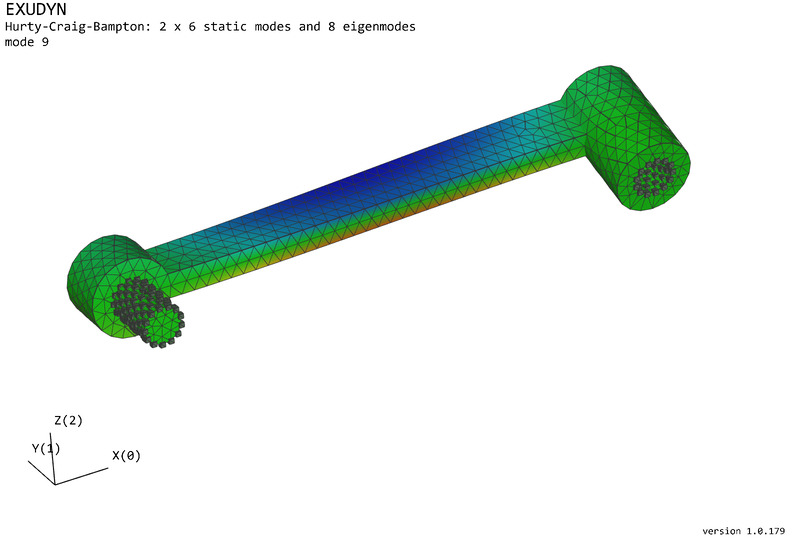
\includegraphics[width=5cm]{figures/modesHinge/HCBmodesHingeStaticBrotX}
  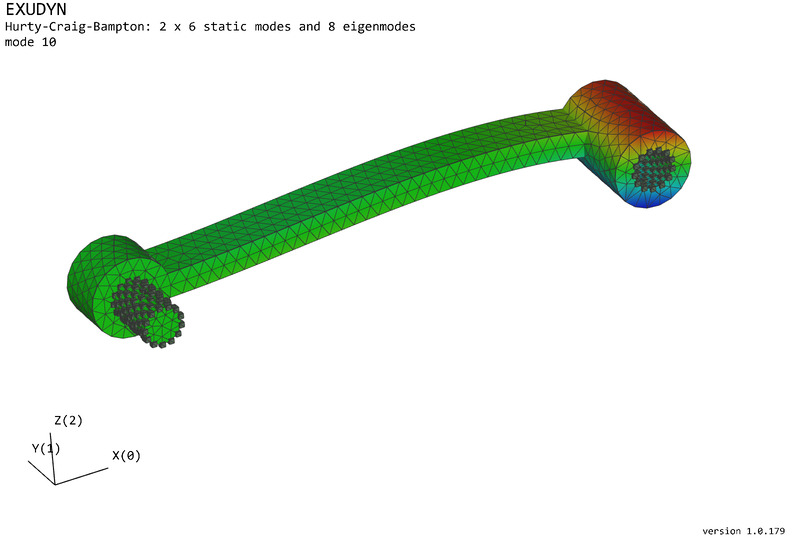
\includegraphics[width=5cm]{figures/modesHinge/HCBmodesHingeStaticBrotY}
  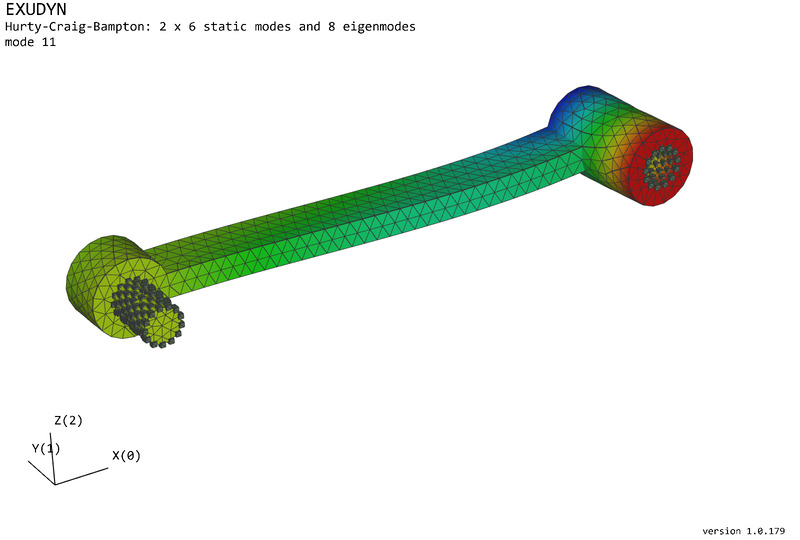
\includegraphics[width=5cm]{figures/modesHinge/HCBmodesHingeStaticBrotZ}
  \end{center}
  \caption{Static modes for bushing rigid body interface, using Hurty-Craig-Bampton method; top three images show (x,y,z)-translation modes, bottom three images show (x,y,z)-rotation modes; contour color represents norm of displacements.}
	\label{fig_hingePartStaticModesB}
\end{figure}
%++++++++++++++++++++++++

%++++++++++++++++++++++++
\begin{figure}[tbph]
  \begin{center}
  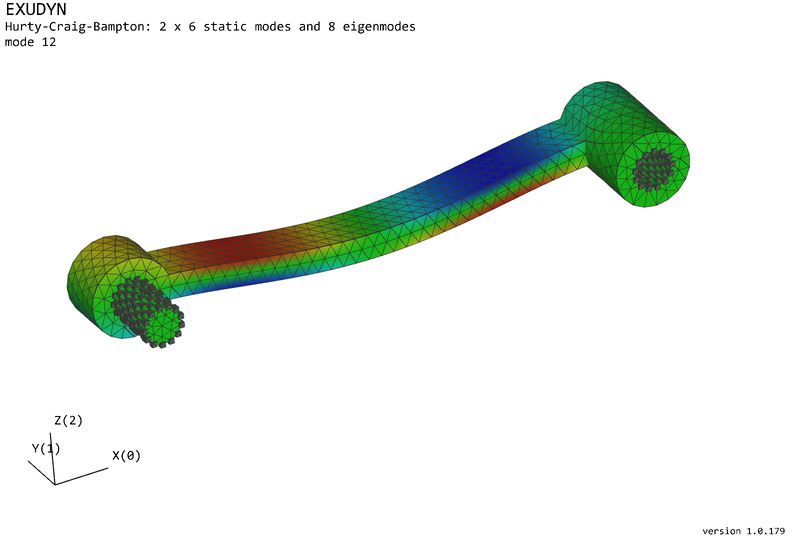
\includegraphics[width=4cm]{figures/modesHinge/HCBmodesHingeEigenmode0}
  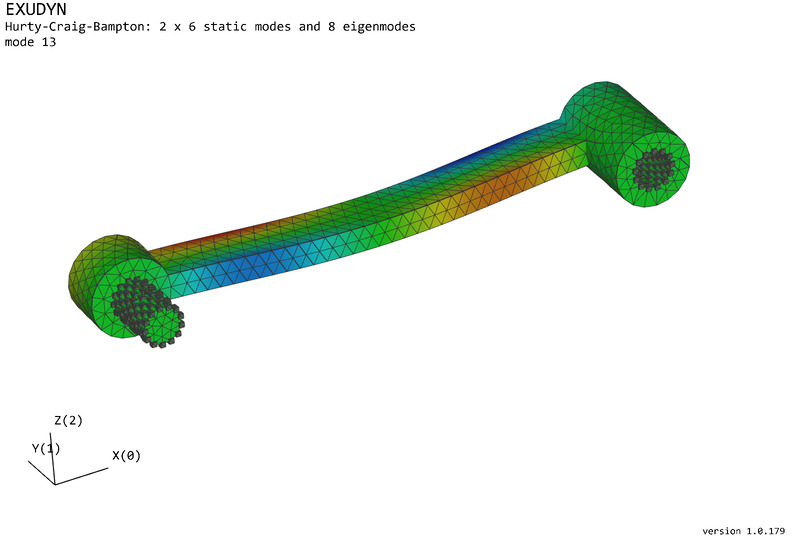
\includegraphics[width=4cm]{figures/modesHinge/HCBmodesHingeEigenmode1}
  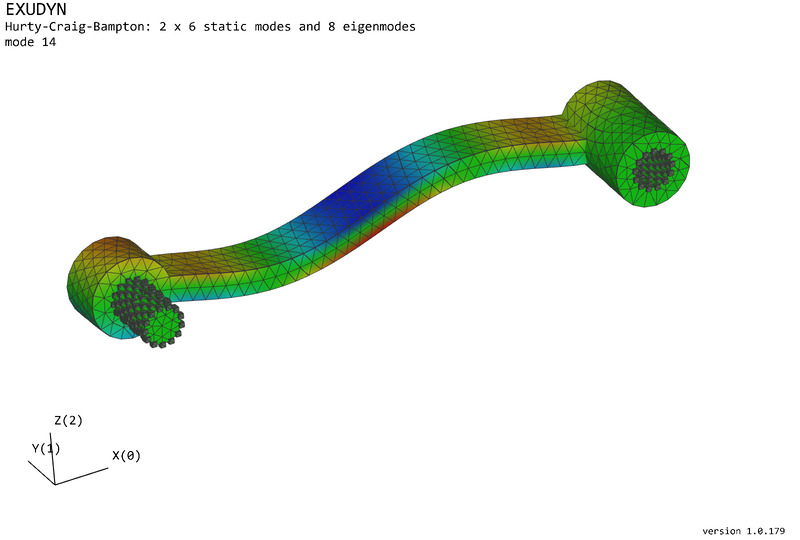
\includegraphics[width=4cm]{figures/modesHinge/HCBmodesHingeEigenmode2}
  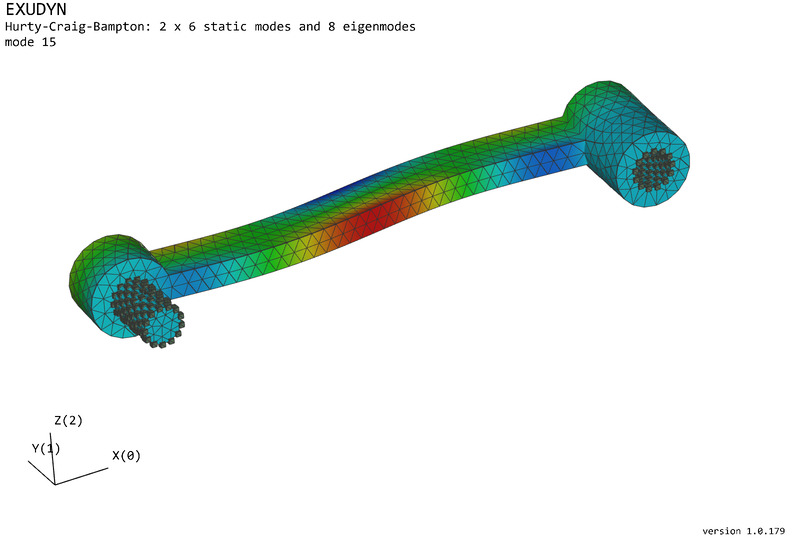
\includegraphics[width=4cm]{figures/modesHinge/HCBmodesHingeEigenmode3}\\
  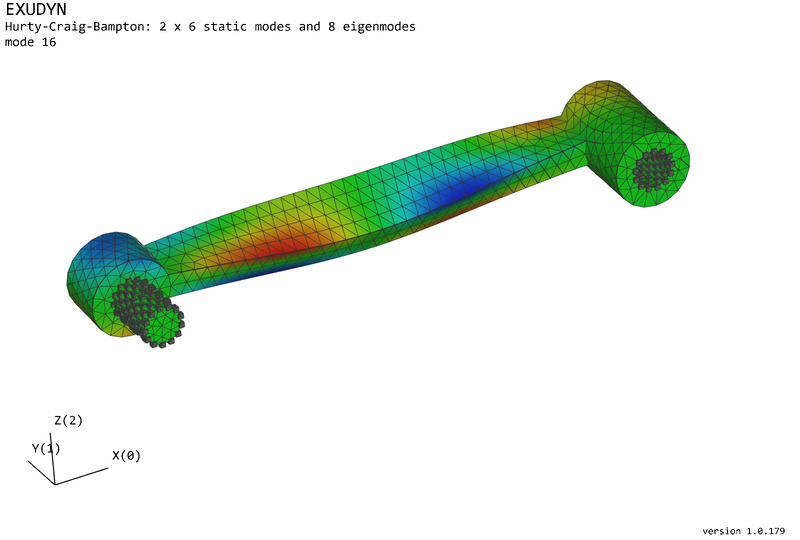
\includegraphics[width=4cm]{figures/modesHinge/HCBmodesHingeEigenmode4}
  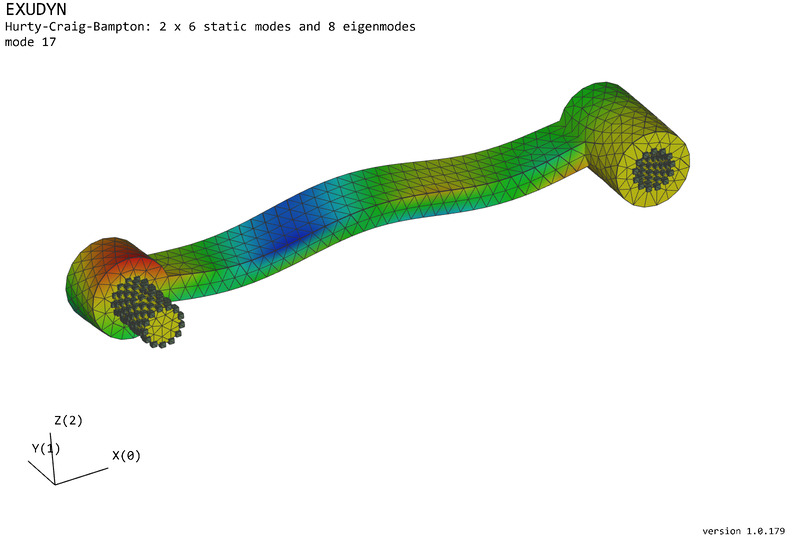
\includegraphics[width=4cm]{figures/modesHinge/HCBmodesHingeEigenmode5}
  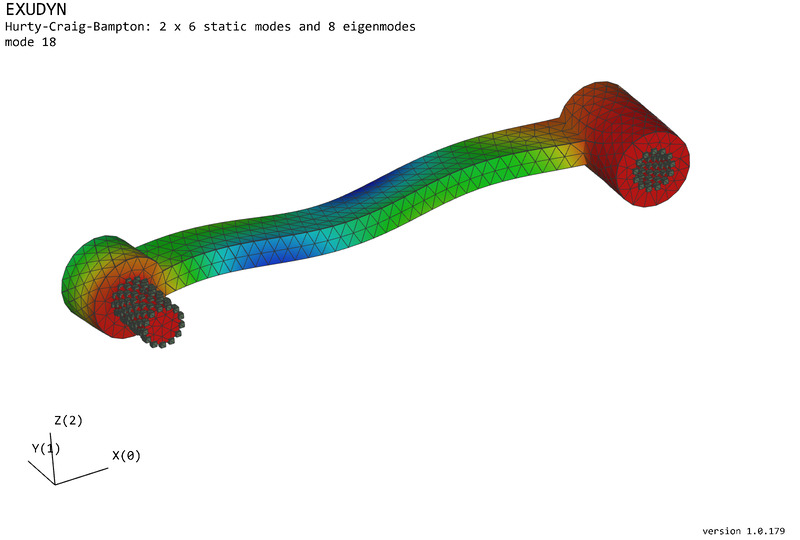
\includegraphics[width=4cm]{figures/modesHinge/HCBmodesHingeEigenmode6}
  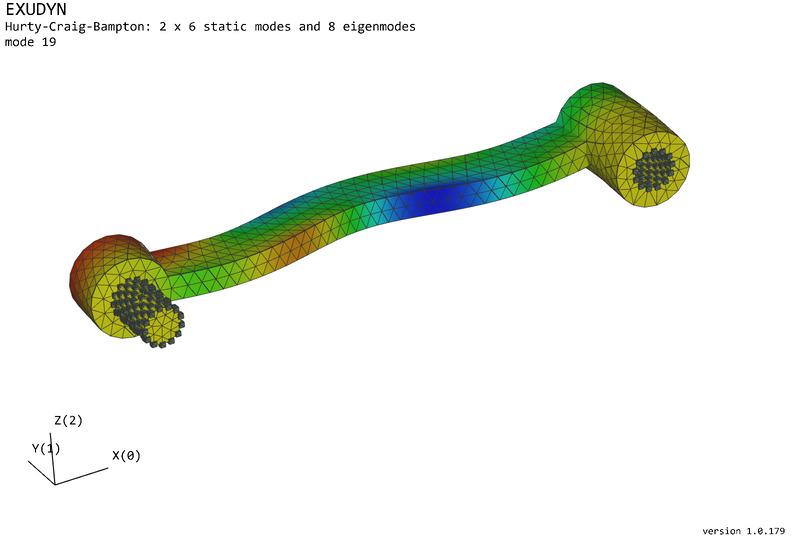
\includegraphics[width=4cm]{figures/modesHinge/HCBmodesHingeEigenmode7}
  \end{center}
  \caption{Eigenmodes for fixed-fixed case, resulting from Hurty-Craig-Bampton method; contour color represents norm of displacements.}
	\label{fig_hingePartFixedFixedModes}
\end{figure}
%++++++++++++++++++++++++

